\documentclass[12pt]{article}

%Filter Warning messages, otherwise it would stuff like
\usepackage{silence}
%Disable all warnings issued by latex starting with "You have..."
\WarningFilter{latex}{You have requested package}

%Allgemeine Einstellungen

%Abstände
\usepackage[a4paper,left=3cm,right=3cm,top=3cm,bottom=3.5cm,headsep=12pt]{geometry}%Bottom extra 0.5cm für Footer

%Deutsches Sprachpacket
\usepackage[german,ngerman]{babel}

%For synmbols like \degree
\usepackage{gensymb}

%Times New Roman
\usepackage{mathptmx}

%Titelseite einbinden
\usepackage{pdfpages}

%1.5-Zeilenabstand
\usepackage[onehalfspacing]{setspace}

%Stil der Überschriften, siehe ueberschriften.sty
\usepackage[numeric]{styPackages/ueberschriften}

%Stil des Inhaltsverzeichnisses, siehe inhaltsverzeichnis.sty
\usepackage[numeric]{styPackages/inhaltsverzeichnis}

%Abkürzungsverzeichnis, siehe abk_verzeichnis.sty
\usepackage{styPackages/abk_verzeichnis}

%Stil der Fußzeilen, siehe fusszeilen.sty
\usepackage{styPackages/fusszeilen}

%Literaturverzeichnis und Zitate, siehe literatur.sty
\usepackage{styPackages/bibliography}

%Stil für Header und Footer, siehe header_footer.sty
%Wenn nicht erwünscht, müssen auch die Befehle \frontmatter, \mainmatter auskommentiert werden
\usepackage{styPackages/header_footer}

%Stile für Code-Ausschnitte, siehe codes.sty
\usepackage{styPackages/codes}

%Stile für Anhänge, Bilder, ...
\usepackage{styPackages/anhang}

\usepackage{styPackages/html}

%Silbentrennung (manche Worte werden am Zeilenende nicht getrennt, diese müssen dann nachgetragen werden)
\usepackage[T1]{fontenc}
\hyphenation{öf-fent-lich-en}

%DEBUGGING (Zeigt Boxen an)
%\usepackage{showframe}
\setlength{\skip\footins}{12pt}

\usepackage{makecell}
\usepackage{placeins}

%Anführungszeichen
\usepackage{csquotes}
\MakeOuterQuote{"}

%[H]-Placing
\usepackage{float}

\usepackage{verbatimbox}

\addto\captionsngerman{\renewcommand{\figurename}{Abb.}}
\addto\captionsngerman{\renewcommand{\tablename}{Tab.}}

%Tabellen oder Bilder mit Textumfluss
\usepackage{wrapfig}
\usepackage{etoolbox}
\BeforeBeginEnvironment{wraptable}{\setlength{\intextsep}{1pt}}
\usepackage[justification=centering]{caption}

%Helvetica font
\usepackage{helvet}
%\renewcommand{\familydefault}{\sfdefault}

%Bookmarks and querverweise
\newcounter{dummy}
\usepackage[hidelinks,bookmarks=true]{hyperref}
\usepackage{bookmark}

%Linebreaks Bib und URL
\usepackage[copyfonts,activate={true,nocompatibility},final,tracking=true,kerning=true,spacing=true,factor=1000,stretch=10,shrink=10]{microtype}
\SetExpansion
[ context = sloppy,
  stretch = 30,
  shrink = 60,
  step = 5 ]
{ encoding = {OT1,T1,TS1} }
{ }

\urlstyle{same}

\renewcommand\UrlFont\itshape

\usepackage{xurl}

\begin{document}

\renewcommand{\mytitle}{Dokumentation\\Deutsch}%Titel für oben links
\renewcommand{\myauthor}{Max Mustermann}%Name für unten links
\renewcommand{\headheight}{27pt}%Bei Mehrzeiligem Titel muss Headerhöhe angepasst werden

\setPlainPageStyle{\mytitle}{\nouppercase\plaintitle}{\myauthor}{\thepage}

\setMainPageStyle{\mytitle}{\nouppercase\parttitle}{\myauthor}{\thepage}

%\includepdf[pages={1-}]{titelseite.pdf}

\frontmatter%Stil des Headers/Footers ändern

\pagenumbering{Roman}

\addcontentsline{toc}{part}{Abkürzungsverzeichnis}%Abk-Verz. ins Inhaltsverzeichnis
\printabbreviations%abk_verzeichnis.sty
\clearpage
\renewcommand{\plaintitle}{Abbildungsverzeichnis}
\addcontentsline{toc}{part}{Abbildungsverzeichnis}
{\def\makebox[#1][#2]#3{#3}%
    \listoffigures
}
\clearpage
\renewcommand{\plaintitle}{Tabellenverzeichnis}
\addcontentsline{toc}{part}{Tabellenverzeichnis}
{\def\makebox[#1][#2]#3{#3}%
    \listoftables
}
\clearpage
\renewcommand{\plaintitle}{Inhaltsverzeichnis}%Titel für oben Rechts
%Defbox, damit gepunktete Linie bis zur Zahl geht
{\def\makebox[#1][#2]#3{#3}%
    \tableofcontents
}

\addtocontents{toc}{\vspace{24pt}}%Freiraum im ToC

\clearpage
\mainmatter%Stil des Headers/Footers ändern
\pagenumbering{arabic}

\part{Einleitung}
Willkommen bei \textit{ThesorTeX}! In diesem Dokument wird beispielhaft gezeigt, wie du die Vorlage und das Tool verwenden kannst. Schaue gern auch ins FAQ auf der Website.\\
Für das Verständnis dieser Vorlage und des Tools werden gewisse Vorkenntnisse in \textit{LaTeX} vorausgesetzt. Falls du etwas mal nicht verstehst, google es einfach mal, vielleicht findest du dann schon Antworten. Bei Problemen mit der Vorlage oder dem Tool, lege sonst gern ein Issue in \href{https://github.com/TimoSto/ThesorTeX/issues}{Github} an.

\part{Verwendung der Vorlage}
Die Vorlage steht unter \url{https://thesortex.com/#/downloads} als ZIP-Datei zum Download bereit. Wenn du diese entpackst, solltest du folgende Struktur sehen:
\begin{itemize}
\setlength\itemsep{.15em}
\item \textbf{data/...}: Diese Dateien sind nur wichtig, wenn du das Tool zum Literaturmanagement verwenden möchtest. Ansonsten kannst du diesen Ordner löschen oder ignorieren.
\item \textbf{styPackages/...}: In diesem Ordner liegen Style-Dateien für die Vorlage. Die Style-Deklarationen könnte man auch in der \textit{main.tex} direkt schreiben, allerdings würde diese dann zu lang werden.
\item \textbf{abkuerzungen.csv}: Hier werden die Abkürzungen aufgeführt, welche in deiner Arbeit gelistet werden sollen. Du kannst die einfach durch ein Semikolon separiert ergänzen.
\item \textbf{bib{\_}entries.csv}: Hier werden deine Literatureinträge im CSV-Format aufgeführt. Auch diese Datei ist primär für die Nutzung mit dem Tool gedacht. Du kannst sie aber grundsätzlich auch ohne nutzen.
\item \textbf{citedKeys.csv}: Angenommen, du hast einige Einträge in deinem Literaturverzeichnis, die nie zitiert werden. Mit dieser Liste kannst du sie aus dem Literaturverzeichnis raushalten, ohne den Eintrag selbst zu verlieren.
\item \textbf{main.tex}: Hier spielt sich die meiste Musik ab! Denn hier schreibst du deinen Text, fügst Listen, Bilder oder Tabellen ein und rufst Zitate auf. Mehr dazu weiter unten.
\end{itemize}

\section{Wie kann ich die Nummerierung der Überschriften ändern?}
Die Nummerierung kann rein numerisch oder alphanumerisch erfolgen:
\begin{center}
\begin{figure}[!h]
  \centering
  \begin{minipage}[b]{0.4\textwidth}
    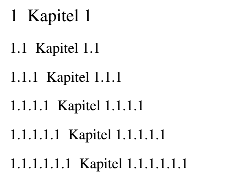
\includegraphics[width=\textwidth]{images/numericChapters.png}
    \caption{Numerische Zählung}
  \end{minipage}
  \hfill
  \begin{minipage}[b]{0.4\textwidth}
    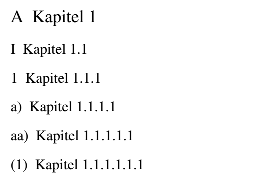
\includegraphics[width=\textwidth]{images/alphaNumericChapters.png}
    \caption{Alphanumerische Zählung}
  \end{minipage}
\end{figure}
\end{center}
\noindent Der Wechsel erfolgt über den Parameter in folgenden Packages:
\begin{lstlisting}
\usepackage[numeric]{styPackages/ueberschriften}
\usepackage[numeric]{styPackages/inhaltsverzeichnis}
\end{lstlisting}
bzw.
\begin{lstlisting}
\usepackage[alphaNumeric]{styPackages/ueberschriften}
\usepackage[alphaNumeric]{styPackages/inhaltsverzeichnis}
\end{lstlisting}

\section{Wie kann ich die Kopf- und Fußzeile ändern?}
In der Kopf- und Fußzeile finden insgesamt vier Informationen Platz. In der Stadnard-Konfiguration sind dies:
\begin{itemize}
\item Oben links: Der Titel deiner Arbeit
\item Oben rechts: Der Titel des aktuellen Ober-Kapitels (\textit{\textbackslash part})
\item Unten links: Dein Name
\item Unten rechts: Die aktuelle Seitenzahl
\end{itemize}
Aber das kannst du ganz einfach ändern. Die Konfiguration für diese Arbeit ist:
\begin{lstlisting}
\renewcommand{\mytitle}{Dokumentation\\Deutsch}%Titel für oben links
\renewcommand{\myauthor}{Max Mustermann}%Name für unten links
\renewcommand{\headheight}{27pt}%Bei Mehrzeiligem Titel muss Headerhöhe angepasst werden

\setPlainPageStyle{\mytitle}{\nouppercase\plaintitle}{\myauthor}{\thepage}

\setMainPageStyle{\mytitle}{\nouppercase\parttitle}{\myauthor}{\thepage}
\end{lstlisting}
Du fragst dich vielleicht, warum es zwei verschiedene Styles gibt. Der \textit{MainPageStyle} ist für den Textteil gedacht. Oben rechts steht dort der Titel des aktuellen Oberkapitels (\textit{\textbackslash part}/\textit{\textbackslash parttitle}). Im \textit{PlainPageStyle} steht dort ein Wert, der frei von dir gewählt werden kann. Dies wird z.B. für das Inhaltsverzeichnis verwendet.\\
Du kannst beide Stile nach deinen Wünschen anpassen:
\begin{lstlisting}
\setPlainPageStyle{OBEN LINKS}{OBEN RECHTS}{UNTEN LINKS}{UNTEN RECHTS}

\setMainPageStyle{OBEN LINKS}{OBEN RECHTS}{UNTEN LINKS}{UNTEN RECHTS}
\end{lstlisting}
Der Wechsel zwischen den beiden Stilen erfolgt über die Befehle \textit{\textbf{\textbackslash frontmatter}} und \textit{\textbf{\textbackslash mainmatter}}.

\section{Wie kann ich Abkürzungen im Abkürzungsverzeichnis ergänzen?}
Das Abkürzungsverzeichnis wird aus der Datei \textbf{\textit{abkuerzungen.csv}} ausgelesen. Dort kannst du deine Abkürzungen in folgendem Format aufführen:
\begin{quote}
\textit{\textbf{Abk};\textbf{Bed};}\\
\textit{Z.B.;Zum Beispiel;}\\
\textit{...}
\end{quote}

\section{Wie kann ich Literatureinträge erstellen?}
\begin{quote}
Es wird empfohlen, hierfür das Literaturmanamement-Tool zu verwenden. Grundsätzlich geht es aber auch ohne.
\end{quote}
Um diese Frage zu beantworten, muss etwas weiter ausgeholt werden. Ein Literatureintrag hat drei Eigenschaften:
\begin{itemize}
\item Einen eindeutigen Schlüssel
\item Eine Kategorie
\item Eine Liste von Feldern (Textwerte)
\end{itemize}
Die Einträge werden auf der Datei \textit{bibEntries.csv} ausgelesen. Für jeden Eintrag wird dann abhängig von der Kategorie ein Literatureintrag bzw. Zitat erstellt.\\
Eine Kategorie hat folgende Eingenschaften:
\begin{itemize}
\item Einen eindeutigen Namen
\item Eine Liste an Feldern fürs Literaturverzeíchnis
\item Eine Liste an Feldern für Zitate
\end{itemize}
Ein Feld wiederum hat folgende Eigenschaften:
\begin{itemize}
\item Einen Namen
\item Einen Prefix und Suffix
\item Einen Stil (kursiv oder normal)
\end{itemize}
Die TeX-Definition der Einträge im Literaturverzeichnis und der Zitate findet sich in \textit{styPackages/bibliography.sty}. Schauen wir uns beispielhaft mal die Kategorie \textit{CitaviArticle} an:
\begin{lstlisting}
\newcommand{\printCitaviArticle}[0]{%
    \hangindent=\bibparindent%
    \parindent 0pt%
    \hangafter=1%
    \argI (\argII): \textit{\argIII} In: \textit{\argIV} \argV, \argVI%
    \\%
    \vspace{-12pt}%

}
\end{lstlisting}
Dieser Befehl sorgt zunächst dafür, dass der Text ab der zweiten Zeile eingeschoben ist. Dann werden die Felder des Eintrags in dem für der Kategorie festgelegten Format ausgegeben.\\
Zitate werden prinzipiell nach demselben Schema definiert:
\begin{lstlisting}
\newcommand{\citeCitaviArticle}[0]{%
    \argVII (\argII), %
}
\end{lstlisting}
Hier wird zunächst das Feld an Stelle sieben ausgegeben, welches im Literatureintrag nicht vorhanden ist. Das kann z.B. der Nachname des Autors sein, während im Literaturverzeichnis der vollständige Name steht. Als nächstes wird Feld 2 ausgegeben. Dieses stimmt mit dem Literaturverzeichnis überein. Das kann z.B. die Jahreszahl sein, welche im Literaturverzeichnis und in Zitaten denselben Wert hat. Das Format kann sich allerdings unterscheiden, sofern du das möchtest.\\
Ein Eintrag in \textit{bibEntries.csv} für die Kategorie \textit{CitaviArticle} sähe wie folgt aus:
\begin{quote}
testEntry;CitaviArticle;Peter Hase;1999;ThesorTeX - Ein tolles Tool;Zeitschrift\textbackslash\_ xy;S.20-22;https:/doi.org/xyz;Hase;;;;;;;;;;;;;;;;;;;
\end{quote}
Das Ergebnis kannst du im Literatuverzeichnis sehen. Beachte, dass manche Sonderzeichen, wie z.B. \_ von Latex vorbelegt sind und deshalb escaped durch den jeweiligen TeX-Befehl ersetzt werden müssen.\\
Zitieren kannst du diesen Eintrag über den Befehl \textit{\textbackslash citebib\{testEntry\}\{vgl. \}\{S.10\}}.\citebib{testEntry}{vgl. }{S.10} Das zweite und dritte Argument sind dabei optimal, können also auch leer bleiben (\textit{\textbackslash citebib\{testEntry\}\{\}\{\}}).\citebib{testEntry}{ }{ }

\section{Wie kann ich Anhänge hinzufügen und auflisten lassen?}
Anhänge können separat nummeriert ausgegeben werden. Als Überschriften kannst du folgende Befehle verwenden:
\begin{itemize}
\item \textit{\textbackslash anhang}
\item \textit{\textbackslash anhangI}
\item \textit{\textbackslash anhangII}
\end{itemize}
Die Liste der Anhänge kann über folgenden Befehl ausgegeben werden:
\begin{lstlisting}
\listofanhang
\end{lstlisting}

\clearpage
\frontmatter%Stil des Headers/Footers ändern
\renewcommand{\plaintitle}{Literaturverzeichnis}
\pagenumbering{Roman}
\setcounter{page}{5}
\addtocontents{toc}{\vspace{24pt}}
\addcontentsline{toc}{part}{Literaturverzeichnis}%Literatur-Verz. ins Inhaltsverzeichnis
\printMyBibliography
\clearpage
\renewcommand{\plaintitle}{Anhang}
\addcontentsline{toc}{part}{Anhang}
{\def\makebox[#1][#2]#3{#3}%
    \listofanhang
}
\clearpage
\anhang{Test Anhang}
Mein erster Anhang

\end{document}